\section{Preparing a Franka demonstration}\label{frankademo}
The intended hardware platform is a Franka arm. Its exact variant and software
remain to be fixed. A local rehearsal uses a pinned Menagerie FR3 model with
seven coupled joints \cite{menagerie}. It is a simulation integration check,
with no libfranka, network, tool, contact task, or learned policy.

Four small joint-motion tasks run with the model's stock position actuators and
with an added ideal model-bias assist, at two integration steps. All 16 runs
complete without simulation warnings or detected contacts. The stock-actuator
hold has about $6.05$ mm of flange error under gravity. The ideal assist removes
that hold error. The assist bypasses the actuator force clamp, so total joint
torque is not certified. Flange scores use world-frame attachment-site position;
they omit orientation. These are model findings, not claims about Franka firmware.

\begin{center}
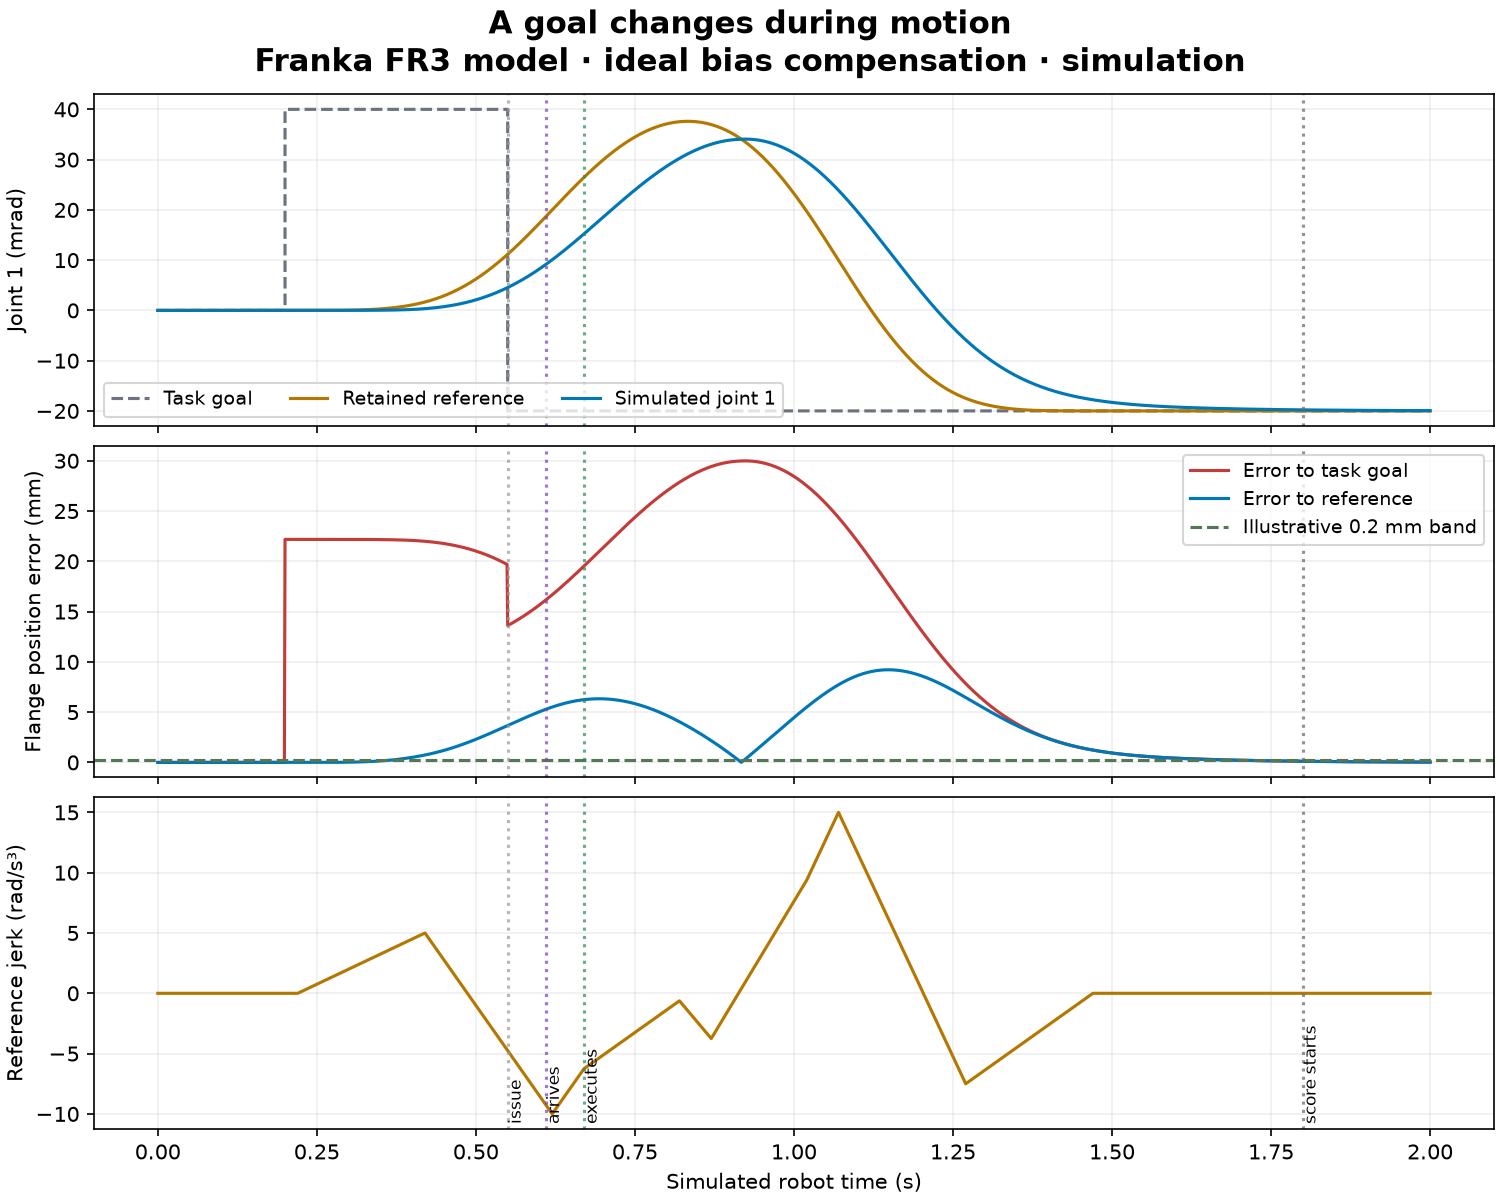
\includegraphics[width=.77\linewidth]{images/franka-rehearsal.png}
\end{center}
\vspace{-.5em}
{\small In this queued reversal, the ideal-assist model meets the sampled final
position band, but its transient reference-tracking error reaches about $9.21$
mm. The scalar tracking theorem therefore cannot simply be attached to this
arm model. A coupled controller/model argument is still needed. The plot shows
simulation, not a hardware result or an independent plant replay.}

\textbf{Execution baseline.} Langella et al. study timing artifacts and an improved
Panda interface, while leaving formal guarantees open \cite{langella}.
Its missing proof is a possible adjacent problem, not evidence that our present
theorem covers it. For a real test, retain issued, received and executed times,
pin controller settings, and measure actual task progress and transient error.
Franka's joint and Cartesian interface conditions also remain separate from
the scalar jerk check \cite{frankalimits}.
